\documentclass[12pt, Arial]{article}
\title{Teaching a Class to Grade Itself using Game Theory}
\author{}%Nick Kaashoek and William Wu
\date{}
\usepackage[margin=1in]{geometry}
\usepackage{parskip}
\usepackage{cite}
\usepackage{graphicx}
\usepackage{amsthm}
\usepackage{wrapfig}
\usepackage[section]{placeins}
\usepackage{enumitem}
\setlength{\parindent}{15pt}
\newtheorem{theorem}{Theorem}
\newtheorem{definition}{Definition}
\begin{document}
\maketitle
\section{Introduction}
Over the past few years, there has been a tremendous increase in the popularity of MOOCs (Massive Open Online Courses), as well the importance of MOOCs to education as a whole. Popular MOOC systems such as Coursera or EdX are well funded, which explains their rapid growth: 60 million dollars were invested in EdX when it started in May of 2012~\cite{canmoocsreducecc}. However, the MOOC's main importance comes from its scalability. MOOCs are able to educate massive numbers of students from anywhere in the world~\cite{makingsenseofmoocs}: By the end of 2012, 1.7 million students had attended a course through Coursera~\cite{swotanalysisofmoocs}. The sheer number of students leads to high student-professor ratios that can reach 150,000:1 in some courses.

High student-professor ratios lead to problems for professors. Professors are simply unable to grade hundreds of thousands of submissions. Currently, two types of solutions are used to remedy the problem: automated grading and peer grading. Automated grading relies on machines to grade assignments. However, machines can only check certain types of answers (i.e. multiple choice), severely limiting the depth of the questions asked~\cite{rightandwrongmoocs}. Even though automated grading for written essays is an active area of research with much recent progress, but the quality and accuracy of such systems is under heavy debate~\cite{automatedsystemssuck}. On the other hand, peer grading can grade any type of question, but a system utilizing it could easily be ``hacked'' by the students~\cite{makingsenseofmoocs}. Although both of these systems are interesting concepts, they are limiting or inaccurate in practice~\cite{howaccurateispeergrading}.

The problem of grading large numbers of submissions is important to solve. Without a solid solution, MOOCs cannot provide efficient feedback for students taking them. This renders the students unable to effectively evaluate the mastery of the course material. Therefore, it is imperative to create an efficient system that enables students to receive feedback to learn effectively.

There have been many attempts at solving such an important problem~\cite{autograding}~\cite{edxsoftware}. However, this work introduces what previous attempts lack: a rigorous mathematical analysis of the system using tools from game theory and mechanism design. This work sets a concrete set of constraints that a grading system must satisfy to mitigate students' incentive to cheat, as well as a concrete benchmark to analyze the efficiency of various systems. Together, these create a concrete measure for evaluating peer grading systems in terms of efficiency (how much time the professor and students spend grading) and fairness for the students (how accurate their final scores are). Having this measurement model is a large contribution in itself, because it allows comparison between different systems. Although a theoretical model cannot predict exactly what will happen in practice, game theory and mechanism design have a history of generally determining mechanisms that work in practice from ones that do not~\cite{AGTbook}. Mechanisms that do not follow game theoretic constraints may work in the short-term, but they will be exploited if possible in the long term~\cite{boycottfinal}.
%[Note from Matt and Christos: 1) mention that coming up with a model is itself a big contribution, because now we can compare the quality of two different mechanisms. 2) Mention that certainly theory is not a perfect predictor of what will happen in practice, but that game theory and mechanism design (and all the assumptions used in this work) have a history of ``calling good mechanisms good and bad mechanisms bad''. Also, solutions that do not satisfy game theoretic constraints may work for a while, but in the long run if a system can be exploited, eventually it will be. See here for an interesting example of this: http://www.insidehighered.com/news/2013/02/12/students-boycott-final-challenge-professors-grading-policy-and-get]

Game theory allows the creation of a unified system of assumptions that simulate student behavior in a class. The grading system can be viewed as a ``game'' where the set of ``rules'' are known to everyone and the ``players'' --- the students --- ``play'' the game in order to get the best possible result. Using the assumptions and rules, game theory can predict how students will behave when they ``play''. This way, mechanism efficiency and effectiveness can be proved, allowing the evaluation of different sets of rules.

The difficulty of the problem lies in finding an incentive for students to spend time to grade assignments of others who they do not care about. Incentivizing students seems simple at first: let the professor give bonus points to students who grade, for example. However, this may not return anything useful because a clever student will just take the points and assign a generic grade (i.e. how can the professor tell the difference between an accurately assigned hundred and randomly awarded 100). The next step would be to implement simple checking: e.g. have each paper be graded by two students who both receive bonus points if their grades match. This case may work if the students are isolated, but the professor still cannot tell the difference between a randomly or sincerely awarded grade. This way, their papers will match those of other clever students, giving them points without grading. These examples show that properly incentivizing graders can be a difficult task. The main purpose of this work is to devise mechanisms which avoid these problems, allowing for work to be distributed efficiently.

As demonstrated by the above examples, the difficulty of the problem lies in the complex behavior of selfish human beings. Because human nature dictates that people will do whatever is in their best interest and may try to outsmart the system, coming up with a strict set of rules to encourage the desired behavior can be quite challenging. A mechanism should be made as simple as possible, but the above examples show that a small amount of simplicity must be sacrificed to obtain a system that cannot be manipulated.

This research topic is made interesting by the complexity of human nature as well as its huge practical value. This paper will cover the thought process of mechanisms leading up to the final mechanism and its implications. All mechanisms and related calculations will be compared in terms of scalability and effectiveness.

We start with a simple model and set of assumptions and gradually build upon this set to achieve an increasingly-realistic model. After every change in assumptions, we create a new mechanism that works effectively and efficiently. By the end of our research, we have contributed a highly realistic and detailed model that other game theorists can build off of to form their own solutions, as well as a set of realistic mechanisms that could be implemented in practice.
\section{Materials and Methods}
\subsection{Scenario}
In order to find a solution to the professor's problem, we consider the case of a single assignment. To apply our solution to an entire class, simply apply it to each assignment separately. In such a ``round'' of grading, there are $n$ students, who each bring one ungraded paper to the professor. These ungraded papers are like the input for a function. Each of these papers, $i$ has an objective score $o_i,~where~ 0\leq o_i \leq 100$. This is the score the professor would give out. Our mechanism then has the students grade the papers in a clever way and output the grades. We identify the students by an index $i$ from $1$ to $n$ and the professor as index $0$.
\subsection{Assumptions}
To create the models that are used to predict the behavior of the students, we use a set process every time. To begin with, we create a set of assumptions. These assumptions are used to explain how students will act in a given situation; for example, one assumption could be that students want good grades. This is a logical assumption that is likely true, as all the assumptions are, and can be used to classify the behavior of the students in a model. The same set of assumptions can be used for multiple models, which will allow us to evaluate different models side by side. To begin with, we create a simple set of assumptions:
\begin{enumerate}[itemsep=0pt, parsep=0pt]
	\item Students want good grades
	\item Doing work makes students unhappy
	\item Students want to be happy
	\item Students only care about their final happiness
	\item The happiness of a student is only affected by their grade and the amount of work they do
\end{enumerate}
To re-express the above in mathematics:
\begin{enumerate}[itemsep=0pt, parsep=0pt]
	\item Students all share a common happiness function, $H(g)$, where \emph{g} represents the grade the students received, and the output is their happiness. w.l.o.g. $H(0)=0$
	\item Students can grade others' work accurately (i.e. they can find $o_i$) but doing so costs one unit of happiness. Therefore after grading $W$ papers, a student's happiness can be expressed as $H(g)-W$
	\item Students want to maximize their final happiness, expressed as $H(g)-W$
	\item Students only care about the expectation of their final happiness, which, put in game theory terms, makes them risk neutral (i.e, if $H(x)=10$ and $H(y)=5$, then getting $x$ and $y$ each with $50$ percent chance, gives a happiness of $7.5$).
	\item The final happiness depends only on the grade assigned to the student and the amount of effort exercised. It does not depend on the score of others
\end{enumerate}

There are two things that need to be considered: the importance of a student's own happiness and the irrelevance of others' grades. Happiness is important because it provides a measure of the combination of the work performed and grade received. The reasoning for not caring about friends is due to the relatively low impact they have on someone's grades and happiness. If a student has 100 friends in a class of 150,000, the chance that he will ever have the opportunity to affect the grades of his friends is tiny. For simplicity, we ignore this tiny probability and assume it is 0.

\subsection{Objective}
The goal of the system is to make sure that every student gets the most happiness when they correctly grade every assignment they are given to grade. Without this property, a system becomes extremely unpredictable. In other words, no student can deviate from the desired behavior to improve his or her happiness. In math terms, if by acting honestly student $i$ grades $w_i$ papers and gets a grade of $g_i$ there should not be any way for the student to spend $w'_i$ units of effort and get a score $g'_i$ where $H(g'_i)-w'_i > H(g_i)-w_i$.

\subsection{Benchmark}
%Efficiency objective%
A benchmark that will allow different mechanisms to be compared is vital to the iterative process of mechanism development. Mechanisms should be compared in terms of the relative happiness of people --- which can be expressed as a function of work done --- as well as the accuracy of the grades produced. Therefore, the benchmark becomes the maximum work assigned to any student plus the maximum deviation of student assigned grades to the correct grades, so that a lower scoring mechanism produces a more desirable outcome. In mathematical terms, we want to minimize the function $max_{i \ge 1} |H(g_i)-H(o_i)| + max_{i \ge 0} w_i$ in the worst possible case. This benchmarking function is known as the \emph{Objective function}, which we will reference in our research.

When creating this benchmark, there are 2 things that need to be considered: accuracy and workload. Accuracy is important because if we do not care, then we could give everyone a 100, which, as explained earlier, is a terrible mechanism. Secondly, ignoring the amount of work done means the professor grade can everything. This is bad because it makes the professor extremely unhappy.

In our case, we use the \emph{maximum} deviation and the \emph{maximum} work done. The reason why we do not use the\emph{sum} of the deviations or the \emph{sum} of work done is the following. Consider these two cases for the maximum deviation of the grade assigned by the mechanism to the hypothetical professor-given grade. Note that the grade the student receives at the end is not necessarily that given by their peers.
\begin{enumerate}[label=\Alph*, itemsep=0pt, parsep=0pt]
	\item Each of 1000 students should receive a 90, but the mechanism assigned a 91 to each of them. Maximum deviation is 1, sum is 1000.
	\item Each of 1000 students should receive a 90. One person is assigned a 0, while everyone else is assigned a 90. Maximum deviation is 90, sum is 90.
\end{enumerate}
Clearly, case A is better than case B. The smaller maximum deviation for case A reflects this.
For the maximum work done, consider the the following cases:
\begin{enumerate}[label=\Alph*, itemsep=0pt, parsep=0pt]
	\item The professor grades 1000 papers. Maximum work is 1000, sum is 1000.
	\item Each of 1000 students grades 2 papers. Maximum work is 2, sum is 2000.
\end{enumerate}
This time, case B is intuitively better than case A. Again, the benchmark captures our intuition.

% We now have a well defined problem that we need to solve. Of course the set of assumptions might not be very realistic as we will so we 

Now that we have created a simple set of assumptions and a benchmark, we can create several simple mechanisms, and improve upon them until we are satisfied with a final mechanism. In the improvement process, we gradually refine our assumptions to better represent reality. This means that the original set of assumptions we proposed will change throughout the course of the paper to allow mechanisms to handle more complex yet more realistic situations.

%Repeat above corrections%
\section{Results}
Once the rules and assumptions have been defined and the benchmark determined, different grading mechanisms can be created and tested. This is where mechanism design and game theory comes into play. Mechanism design is used to create a system that satisfies a set of constraints and achieves a certain purpose. Then, game theory is used to mathematically predict student behavior to benchmark such a system. Starting from the simplest and most obvious approaches, various mechanisms were created, tested, and refined upon in an iterative process that spanned several months. The end result is fairly complete, although there are still questions to be answered in future work.

\subsection{Calibration Mechanism}
\label{sec:calibration}

\subsubsection{Process}
First, we design a mechanism that does extremely well in a model defined by our simple and unrealistic assumptions, which we used as a starting point.
One idea is to have the professor choose one paper that he grades. He then distributes this paper to every student, along with a second, ungraded paper. If the students fail to grade the paper the professor graded correctly, they get a 0. If they succeed, they receive their assigned grade.
This is almost exactly the Calibration Mechanism, except we make a small modification. Considering the idea as is, a student whose own grade on the assignment is a 0 has no incentive to grade the paper: Their grade will be a 0 whether or not they grade the paper, so why bother? To cope with this, we pick some minimum grade $m > 0$ and promise every student that they will receive a grade of at least $m$ if they grade the assignment correctly.
By appropriately choosing a value for $m$, all students should behave honestly and the mechanism should output accurate grades while maintaining a low amount of per-person work.
\begin{definition}(Calibration Mechanism)
First, the professor pre-grades a paper $P$. Each student is asked to grade two papers: $P$ and another paper. If the student fails to grade $P$, he or she gets a zero. Otherwise, the student gets the maximum of some minimum value and his or her assigned grade.
\end{definition}
\begin{theorem}
If $m>H^{-1}(2)$, it will be in every student's best interest to grade both papers in the Calibration Mechanism.
\end{theorem}
\begin{proof}
Consider the student $i$.
If all other students behave as desired, student $i$ will be assigned a grade $G=max(m,o_i)$ unless he or she does not grade $P$ correctly.
The happiness of student $i$ grading one paper is $\frac{H(G)}{2}-1$, because the student has a 50\% chance of getting a 0 and a 50\% chance of getting $G$.
If student $i$ grades both papers, his or her happiness will be $H(G)-2$ because he or she is guaranteed to receive $G$ by grading both correctly.
If student $i$ grades neither, his or her happiness will be $0$, because he or she spends no energy and gets a 0.
Therefore, if $H(G) > 2$, then student $i$ will grade both papers. So, for the professor to guarantee that the class use effort and obtain the correct grades, $H(m) > 2$.
Since we chose $m$ to be greater than $H^{-1}(2)$, the previous always holds.
\end{proof}
\emph{This process is summarized in Figure~\ref{fig:calibration} on page~\pageref{fig:calibration}.}

\subsubsection{Benchmark and Remaining Issues}
We now show that the Calibration Mechanism achieves a very low value in our benchmark.
\begin{theorem}
The Calibration Mechanism achieves a benchmark score of 4.
\end{theorem}
\begin{proof}
The teacher expends one unit of effort, each student spends 2, as long as the teacher set the minimum value $m$ high enough.
Everything above $H^{-1}(2)$ will be graded correctly, while everything below it will receive a score of $H^{-1}(2)$.
So, maximum deviation is $H^{-1}(2)$, because this is the score that might be given to someone who deserves a 0. Expressed in happiness units, the value is 2.
\end{proof}

\emph{The benchmark results for the Calibration Mechanism can be seen in Figure~\ref{fig:comparison} on page~\pageref{fig:comparison}, together with results from other mechanisms.}

This mechanism is extremely simple, and relies on the unrealistic assumption that students are unable to communicate with each other. If they were able to, students would be able to figure out which paper is calibrated by checking which one they all share.
%%%%%%%% Go over this section and try to make it similar to the above section. %%%%%%%%
\subsection{Improved Calibration Mechanism}
\subsubsection{Process}
In the calibration mechanism, we assumed that students could not communicate with each other, and therefore could not figure out which of the two papers they were asked to grade was calibrated. For this mechanism, we relax this assumption and instead provide a mechanism that works even if each student can communicate with all other students.
\begin{definition}(Improved Calibration Mechanism)
In this mechanism, we apply the Calibration Mechanism on a larger scale. Every student is put into a cycle. Each student grades the papers of $k$ next students. The professor also grades every $kth$ paper in the cycle, which become the calibrated papers. The same system for assigning grades is used as in the calibration mechanism.
\end{definition}
\begin{theorem}
In this mechanism, students will return accurate grades, even though they can communicate with each other.
\end{theorem}
\begin{proof}
In this scheme, because of the overlapping papers, the students have no better way of figuring out which papers are calibrated than random guessing, even though they can all communicate with each other. As such, there are 3 options for the students. They can grade 0 papers, giving them a happiness of $H(0) = 0$ or grade all the papers they are assigned, giving them a happiness of $H(g) - k$ or they can grade $i$ papers giving them a happiness of $\frac{i}{k} \cdot H(G)-i$. This means that it is always worse to grade $i$, because happiness from grading $i$ is equal to $i$ times happiness for grading 0 plus $i-k$ times happiness for grading $k$.

Even though the students can communicate with one another, they will have no way to determine which paper is calibrated because there are multiple calibrated papers that overlap, and are thus best off grading all the papers. As long as $m > H^{-1}(k)$, the papers will be accurately graded, as before.

\end{proof}
\subsubsection{Benchmark and Remaining Issues}
The amount of work done by the professor is $\frac{n}{k}$. For the students, this number is $k$. The maximum grade deviation is also $k$, for $m > H^{-1}(k)$. Therefore, the benchmark $max(k, \frac{n}{k}) + k$, a potentially higher value than before. The huge problem with this is the high amount of work being done, choosing the optimal value for $k$, which is $\sqrt{n}$. We can see that the benchmark becomes $2\sqrt{n}$.

\emph{The benchmark results for the Improved Calibration Mechanism can be seen in Figure~\ref{fig:comparison} on page~\pageref{fig:comparison}.}
%%%%%%%% Revise this section to be like the above. %%%%%%%%
\subsection{Deduction Mechanism}
\label{sec:deduction}
With this mechanism, we aim to fix the faults of the previous mechanism while retaining the same set of assumptions. Other than reducing the workload, we aim to accomplish the same goals as the improved calibration mechanism.
\subsubsection{Process}
\begin{definition}(Deduction Mechanism)
In this mechanism, each paper is randomly assigned to 2 students. Students deduct as many points as they want, and write a justification for each of them. For each paper graded by students $i$ and $j$, where $i$ took of $x_i$ points and $j$ took off $x_j$, student $i$ receives contribution score $\frac{x_i}{x_i + x_j}$, and $j$ receives $\frac{x_j}{x_i + x_j}$. Students may then choose to appeal their paper's grade if they are unhappy with it, at which point the professor grades it and gives the incorrect grader(s) a 0. To compute the final score for a student, the final grade on the assignment is calculated as follows: 4 points times their contribution score are added or subtracted to $H(g)$. (Then the student's grade is converted from Happiness to an actual score).
\end{definition}
\begin{theorem}
The addition of the contribution score being added or subtracted should encourage graders to honestly grade papers, for fear of losing points and the possible reward.
\end{theorem}
\begin{proof}
The graders have two choices, they can either grade the papers, or not grade them.

If the grader does not grade the paper, what score should he or she give it?

If they take off any points that should not be taken off, the points will surely be refuted by the professor during the regrade.
So if they take off any points, they will get a 0 on the grading assignment because of the professor's punishment.
If the grader gives the paper 100, they might get 0.5 if the other grader also gives it 100. If he gives it anything else, the original grader will get 0. This is much better than a guaranteed zero, so they will give the paper 100.

If the grader does grade the paper, what score should he give it?

Obviously, if the student takes the effort to grade the paper, they will give the paper its true score, because doing anything else either forfeits a higher contribution score, or guarantees a 0 due to the professor's punishment. This means that they are guaranteed at least a contribution score of 0.5, so after grading both of their assigned papers, the graders will get a full contribution score of 1.

Now that we know what the students will do, lets look at what happens when we introduce the grading partner. 

If the student's partner gives the paper a 100, which is the best thing they could do if they do not grade, then
	If they do not grade the paper, they do not use any effort, and their contribution score is 0. So the student's happiness will $H(g) + 4*0 = H(g)$.

If the student grades, he or she uses 1 unit of effort by default, but get the full contribution score of 1. This means that their final happiness is $H(g) + 4\cdot1 - 1 = H(g)+3$.
	
If the partner gives the paper its true grade:
	If the grader does not grade the assignment, they will give it a 100 and so the grader's contribution score is -1. So their happiness is $H(g) + 4\cdot(-1) = H(g)-4$.

If the grader does grade the assignment, they and their partner gave the same grades, so they get a contribution score of 0. This means that their happiness is $H(g) + 4\cdot0 - 1 = H(g)-1$.
	
In both of the above cases, the happiness outputs for honestly grading the paper is higher than the happiness output when not grading the paper. Our assumptions state that students will do whatever makes them happiest, so they will honestly grade the papers.

\end{proof}
\noindent
\emph{This process is summarized in Figure~\ref{fig:deduction} on page~\pageref{fig:deduction}.}
\newline
\emph{The benchmark results for the Calibration Mechanism can be seen in Figure~\ref{fig:comparison} on page~\pageref{fig:comparison}.}
\subsubsection{Benchmark}
In this model, the most work is being done by the students, who each grade 2 papers. In this mechanism, the professor will not perform any work, because students will adhere to the dominant strategy behavior, and honestly grade the paper. This means that no papers will ever reach the professor, so he or she will not have to grade anything. Also, because every student will follow dominant strategy behavior, the maximum deviation from the objective score will be 0, since every student will output accurate grades. This means that the final benchmark is $2+0=2$. This is the lowest out of all the mechanisms so far.
\subsection{Final Assumptions}
Now that we have reached a point far into the research, we have a model that accounts for a very realistic world view. However, the Deduction Mechanism still has some unrealistic parts, primarily the inability to deal with students who are incompetent graders. To address this, we designed a final set of assumptions that more effectively simulate a realistic world.

\begin{enumerate}[itemsep=0pt, parsep=0pt]
	\item When grading, $w_i=0 \oplus w_i=1$
	\item For all students, $g_i \neq o_i$
	\item Students all share a common happiness function, $H(g)$, where $g$ represents the grade the students received, and the output is their happiness. w.l.o.g. $H(0)=0$
	\item Students can grade others' work perfectly but doing so costs one unit of happiness. Therefore after grading $W$ papers, a student's happiness can be expressed as $H(g)-W$
	\item Final happiness is unaffected by other people, only affected by $g_i$ and $w_i$
	\item Students only care about the expectation of their final happiness, which, put in game theory terms, makes them risk neutral
	\item For a given student in $N$, that student has contact with all other students in $N$
\end{enumerate}
\newpage
\section{Illustrations}
{
\noindent
%%%%%%%% Make sure the comparison chart shows 2*sqrt(n) %%%%%%%%
\begin{figure}[!h]
	\centering
		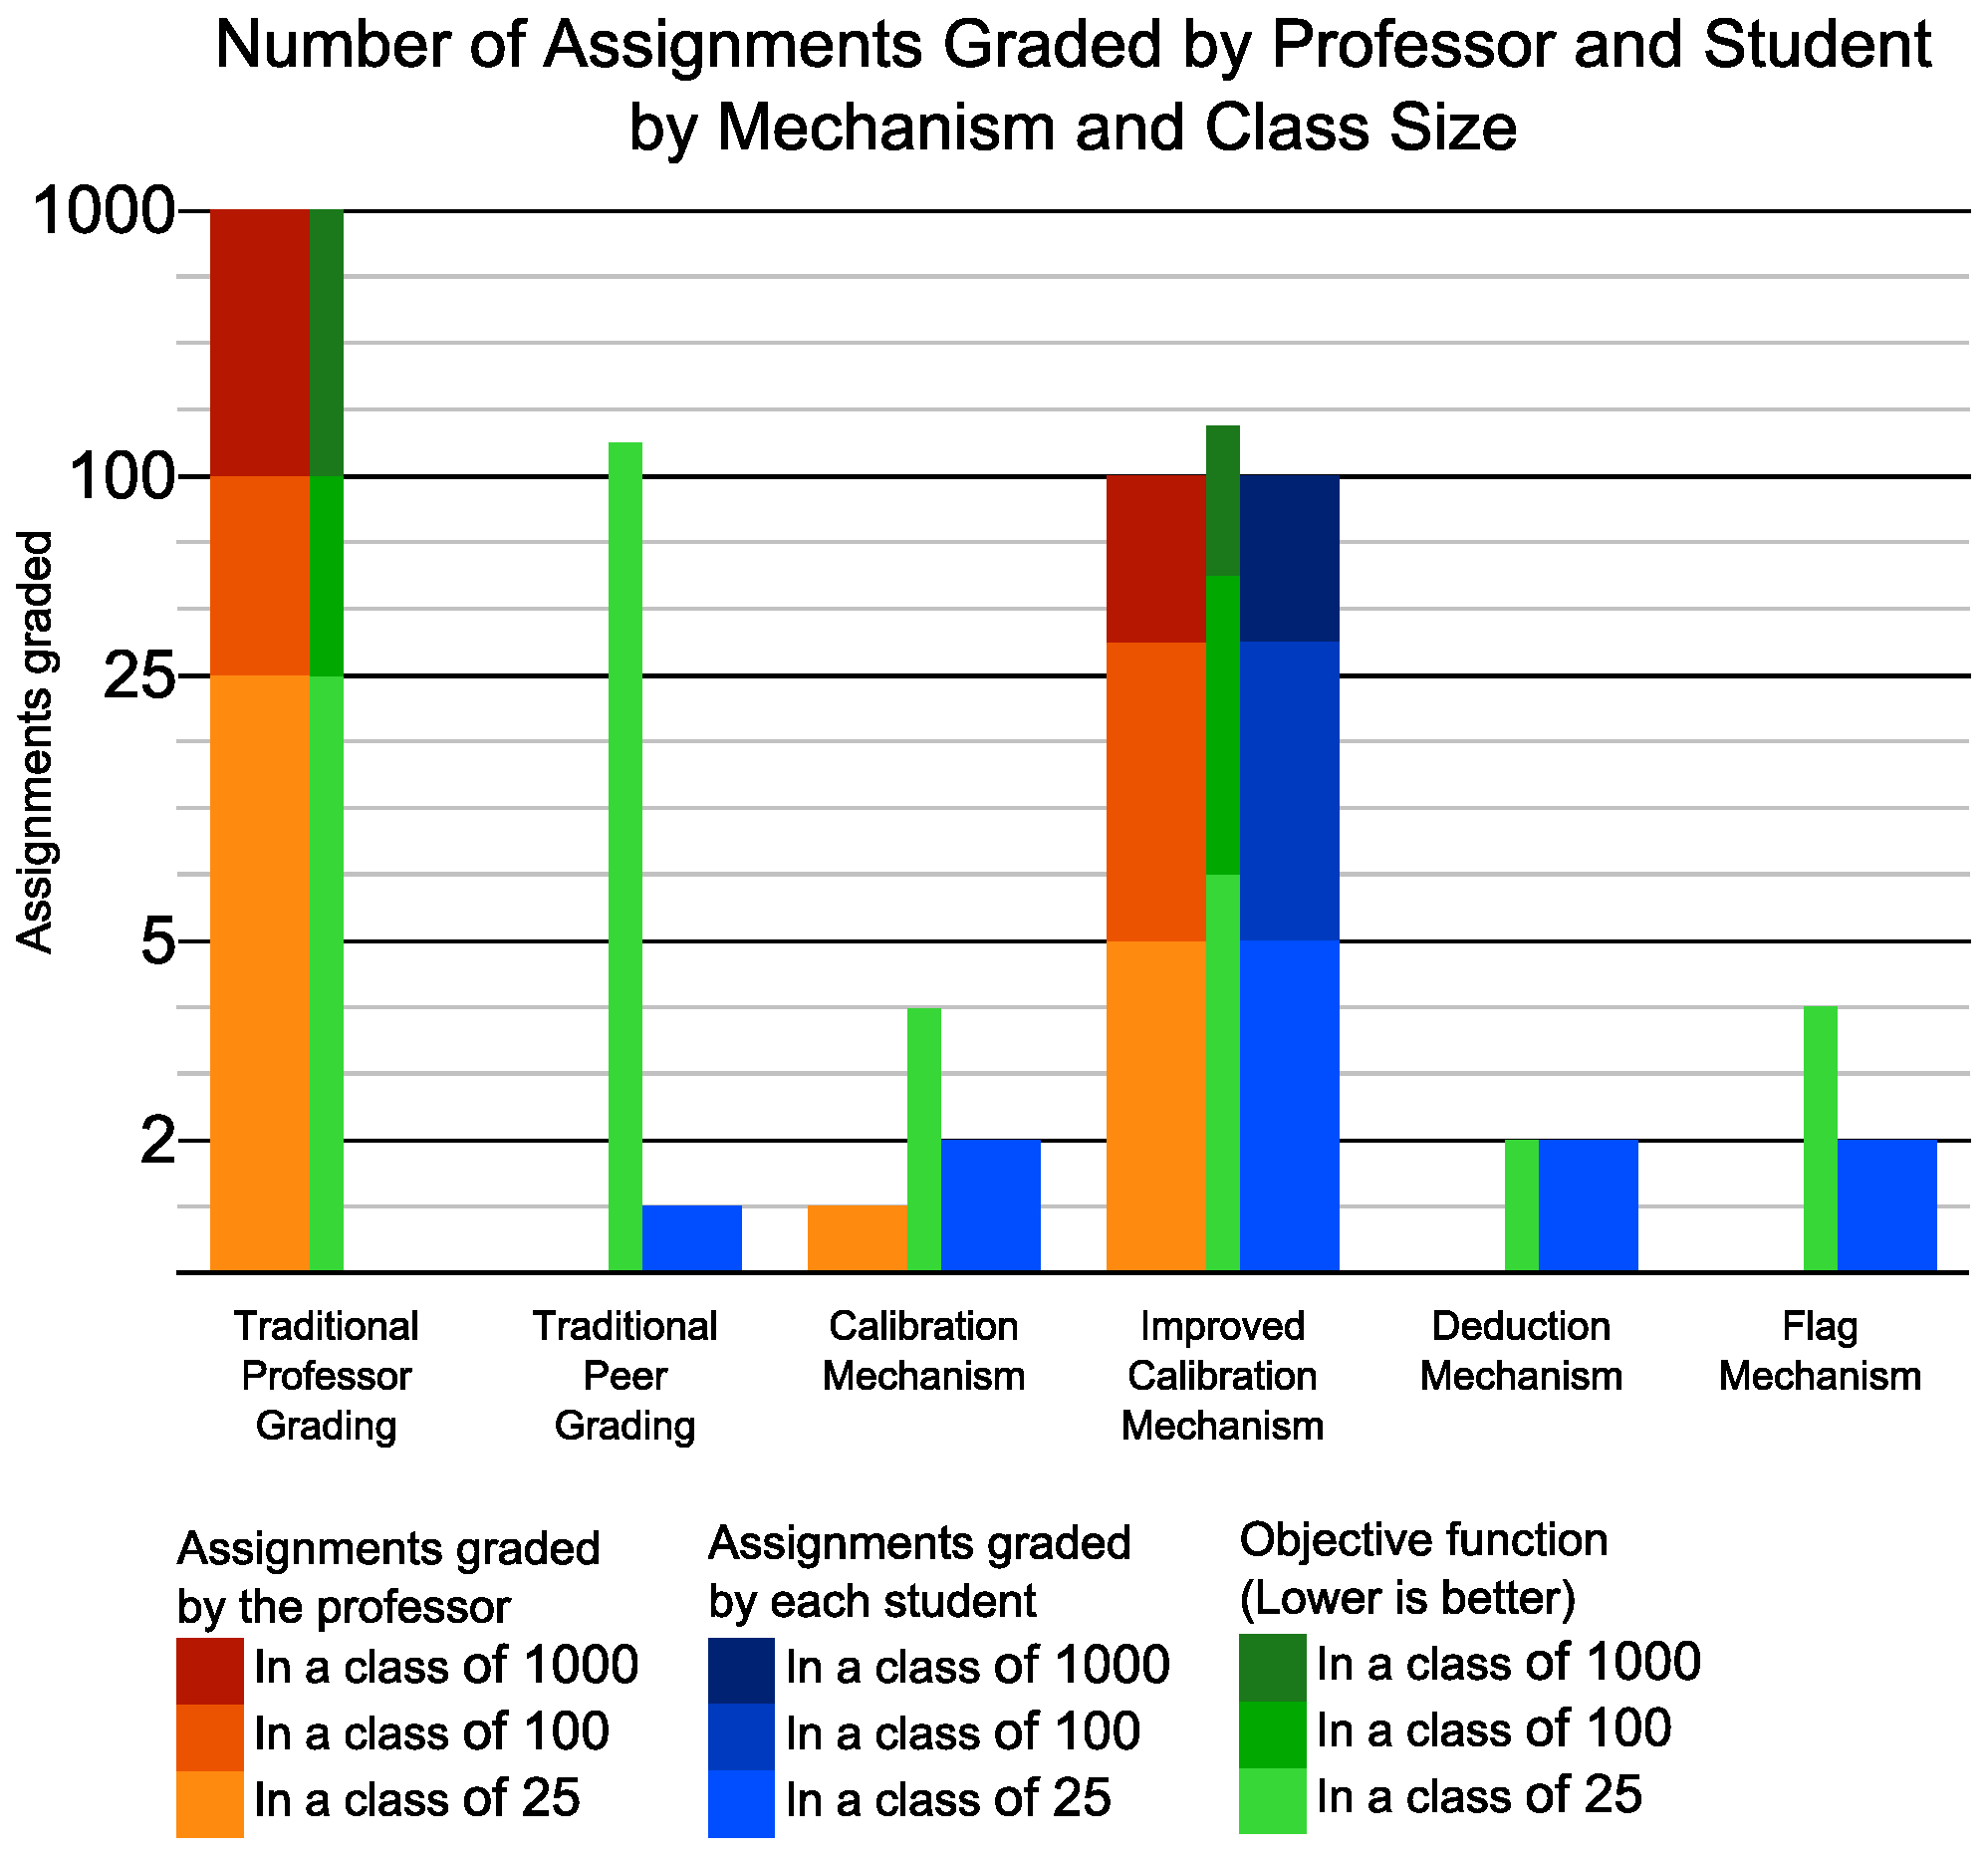
\includegraphics[width=0.75\textwidth]{Comparison.eps}
		\caption {A comparison of mechanisms in terms of effectiveness and scalability.\label{fig:comparison}}
\end{figure}
\begin{figure}
	\centering
		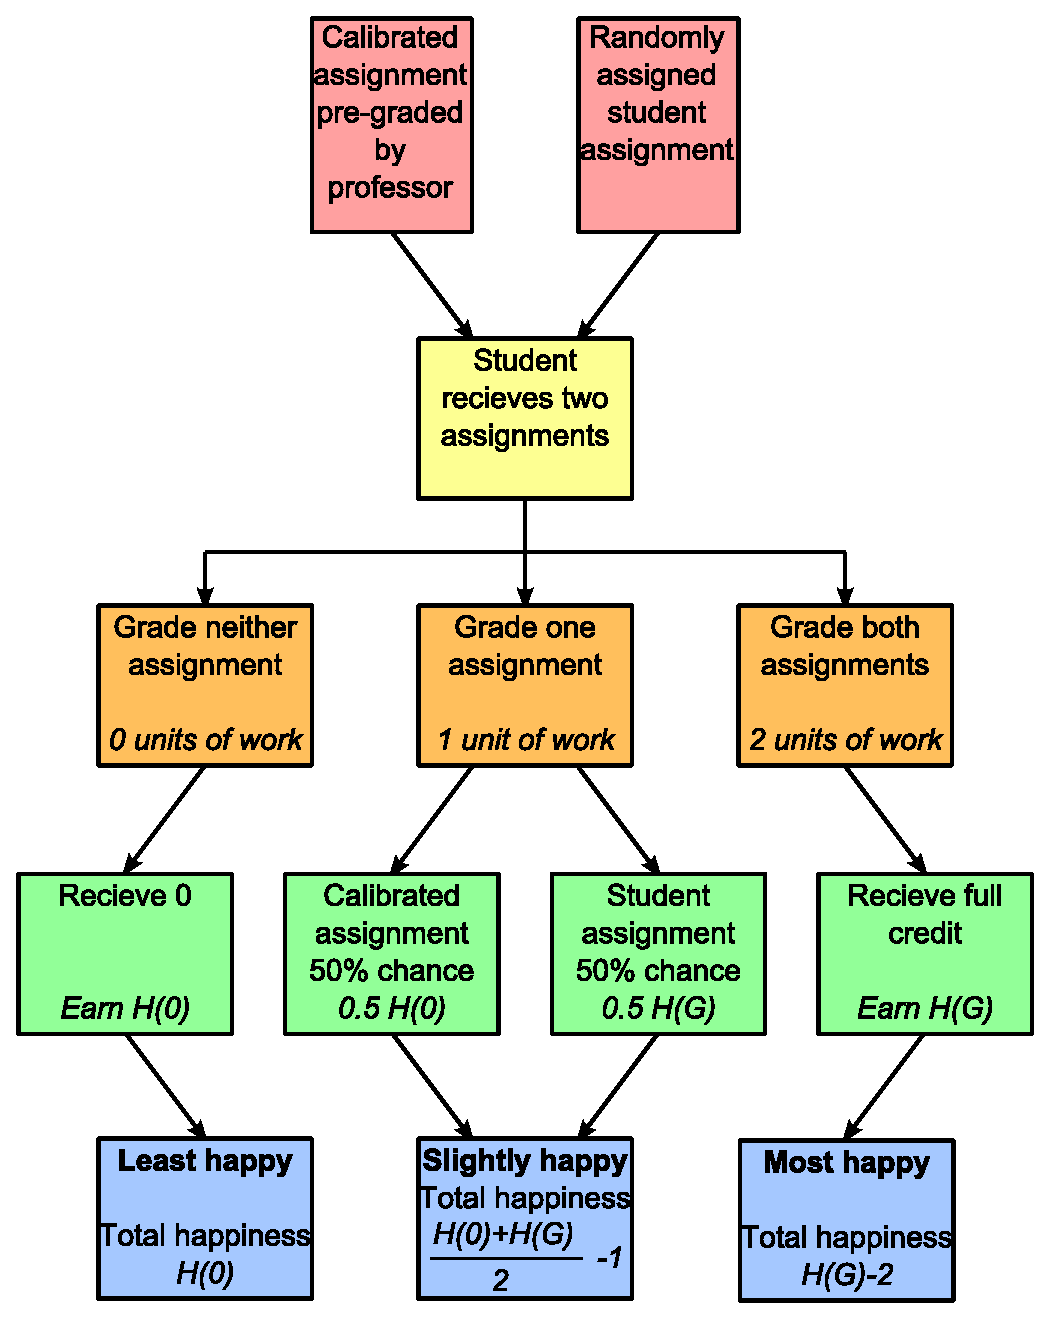
\includegraphics[width=0.75\textwidth]{Flowchart-Calibration.eps}
		\caption {A flowchart of the Calibration Mechanism (Section~\ref{sec:calibration}, page~\pageref{sec:calibration}) from the student perspective.\label{fig:calibration}}
\end{figure}
\begin{figure}
	\centering
		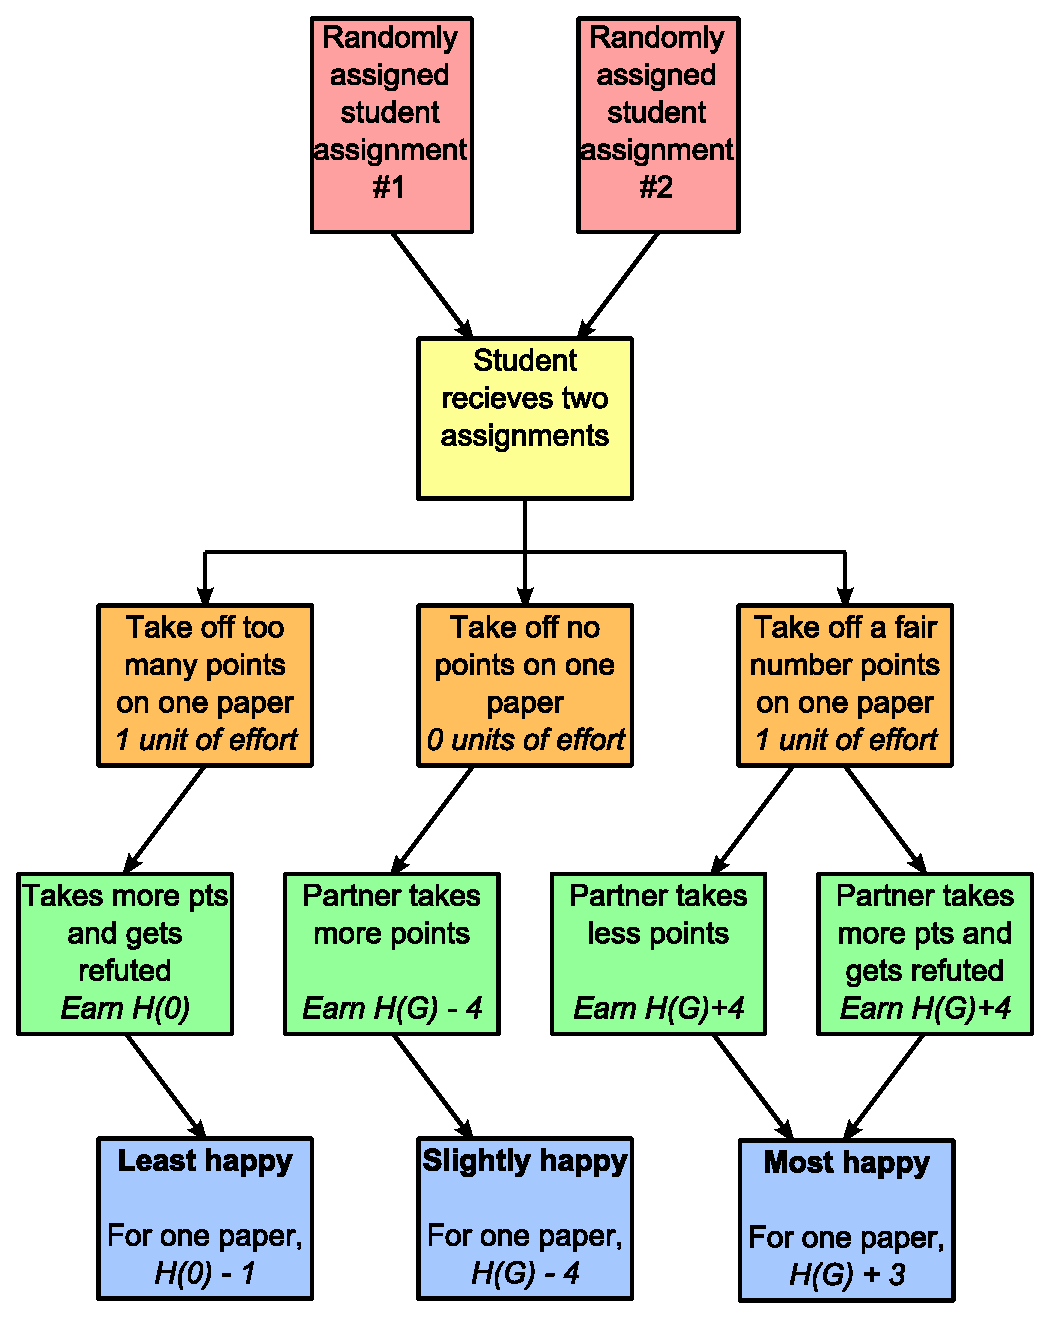
\includegraphics[width=0.75\textwidth]{Flowchart-Deduction.eps}
		\caption {A flowchart of the Deduction Mechanism (Section~\ref{sec:deduction}, page~\pageref{sec:deduction}) from the student perspective.\label{fig:deduction}}
\end{figure}
}
%%%%%%%% Go over this section, make edits and revise. %%%%%%%%
\section{Discussion}
With this research, the goal was to create a mechanism that fulfilled our goal; incentivizing students to play the ``game'' to correctly grade the assignments of other students. The mechanism created by the end of the research was realistic enough to be implemented in a classroom environment where all students are capable of grading others assignments efficiently.

The work done in this research furthers past solutions of grading large numbers of papers, some of which involve creating automated mechanisms that assign non-human grades. These automated solutions, as stated before, often produce unsatisfactory results. By creating a grading mechanism using game theory, we have shown that computers do not need to be relied upon to accurately and efficiently grade papers, leading the way for others to create game-theory-driven solutions to this problem.

By taking the happiness of the students into account, it can be almost guaranteed that these mechanisms are better for the students than automated grading, or any other solutions attempted before. Many student-given complaints express the lack of feedback the students can provide about their grades. This problem, found in systems such as Coursera~\cite{howaccurateispeergrading}, is solved by our mechanisms by allowing the students to appeal their grades and to have multiple rounds of grading. Our mechanisms addresses other commonly expressed problems such as inconsistency of feedback by requiring a reason for every deduction made --- students must take the time to explain any deductions, or why they gave the paper a perfect score.

Besides making the students happier than they are in other peer grading systems, the mechanisms that result from this research also provide more accurate and legitimate grades for the students. In current peer grading schemes, it is easy for students to just ``game'' the system and fake their way through a course. Giving anonymous feedback, for example, does not encourage students to be honest, rather, it gives them a reason to be \emph{dis}honest~\cite{howaccurateispeergrading}. This allows students to dishonestly grade the work of others, as well as just give whomever they want a better grade than that person actually deserves. In our mechanisms, however, these problems are solved by removing anonymity and adding incentives to make students behave honestly, no matter who they are grading.

Aside from fixing many problems that students have with other peer grading systems, our mechanisms also address the unhappiness and inconsistency caused by the grading given out by machines. One key problem that machines have is that they always look at the same thing in a paper, meaning that they can be easily ``gamed''and fooled into thinking something is better than it acutely is~\cite{robogradingproblems}. Not only does this make the system inconsistent, but any student who is lacking something that is in the list of requirements the machine checks for can be unfairly given a poor grade, making them unhappy. By solving both of these problems with the mechanisms that were created, it has been demonstrated the peer grading, at least for the moment, is better for education that automated grading.

Not only do the mechanisms developed in this research improve upon the efficiency of automated grading systems, but they also help to remove the dominance that automated grading has placed on grading large courses. By providing a system that fixes many of the problems with current automated grading systems, these mechanisms help to show that automated grading is not the only way to solve the problem of grading online courses. Because automated grading, at the moment, is not as efficient and robust as it needs to be to prevent students from creating unfair situations, this is something that is necessary to show because automated grading is simply not good enough with today's technology.

By creating a mechanism that is, in theory, more efficient than both current peer grading systems and automated grading systems, it has been shown that there is still room for improvement in the grading of online courses. By showing this, a renewed interest in the field can be created, which could lead to others developing more mechanisms that will improve the general education of students in these courses. As the ultimate goal of this research is to accomplish this, the idea that the mechanisms not only accomplish this, but also open the road for others to do so is a marked success.

With the final mechanism, all of the goals that were set up were accomplished, with only total realism absent from the design. With this final mechanism, it has been shown that it is possible to create a mathematically driven and effective design that can solve a problem that needs to be solved. Not only is this something that has not been done before, but it opens the way for others to build upon this work, something that could eventually lead to the creation of a perfect solution. 

However important the creation of these mechanisms is, arguably more important to the future development of further solutions is the creation of a realistic and robust model. Without a model, many of the mechanisms mentioned would have been impossible to create, and would certainly not work as well as they do. The creation of a model is essential in game theory as it provides the outline for how the ``players''of a given game will act under any set of circumstances. As such, by creating a good model, this research has undergone the trouble of providing a way for anyone to predict how students will behave. 

Not only did this research lead to the creation of a good model, but it also led to the creation of a benchmark. The creation of a benchmark is important because it allows two mechanisms to be compared side by side, and it allows theorists to definitively determine which of these mechanisms is superior. With this, it becomes possible to compare the results of this research to the results of others, and also allows future work to be done by others. Not only does a benchmark allow the research done here to be compared to that of others, but it allows two totally independent mechanisms not derived from this research to be compared, which could lead to a universal system of evaluating peer grading systems.

Both of these are major contributions towards further developments in the field of research this problem takes place in, primarily game theory. By doing so, grading mechanisms across online courses will constantly be able to evolve and improve with contributions from anyone. By creating the benchmark and model, all mechanisms will undergo a uniform set of evaluations that will allow online course systems to determine which system is the best out of any proposals. By doing so, this research has opened up a road for many game theorists to develop and analyze new ideas that will lead to improvements in student happiness and results from online courses.

Due to the numerous possibilities the creation of a model and benchmark can lead to future research, it is clear that they are the most important results gained from this research. Without them, nothing else could have been done, and no future mechanisms could be created that would be able to be analyzed in the same way that these were. Due to the importance of future research in this field, it was imperative that this research led to more solutions in the future, so that the problem that was identified would be quickly and efficiently solved.

Although the models presented by this research are not completely realistic, they do show that there is much room for improvement in the area of grading online courses, and that it is possible to take a strictly mathematical approach at designing a mechanism, and then implementing it using computer science. By showing that this is possible, a huge amount of potential for future research has been opened, primarily due to the creation of a benchmark and model. With these tools, other game theorists can create their own mechanisms, and compare them to those of others around the world.

Aside from improving previous research done in this field, this research also supports the idea that many others have proposed: that peer grading is more efficient than automated grading. When EdX first introduced its automated grading system, many were skeptical of the idea, and had right to be. For this reason, systems such as Coursera have yet to adopt this, and instead default to peer grading. As many people suspected, and as this research confirms, peer grading can indeed be more efficient than automated grading when implemented correctly, simply because the A.I. of current machines cannot handle the many different ways a student can answer an open ended question.

Human judgment has always been superior to that of a machine, and this research continues to support that idea. As powerful as automated grading can be in practice, when it comes to theory, peer grading is simply more efficient. This means that with the right mechanism, such as the ones proposed by this research, so, in practice peer grading should be superior to automated grading. This research has opened doors for game theorists to make improvements to current grading schemes, and also provides mechanisms that are a distinct improvement over current peer and automated grading systems.

As our mechanisms evolve, the benchmark scores yielded by each tends to decrease. However, this is not the case with the Improved Calibration Mechanism, which actually provided a higher benchmark score than the previous mechanism. This stems from the fact that the assumptions were changed, and the mechanism was not. This shows that with a change in assumptions, a new mechanism must be created to address the change, as old mechanisms will often perform badly in new models.

In comparison with more traditional methods of peer grading, our mechanisms performed extremely well, aside from the Improved Calibration Mechanism. \emph{See Figure~\ref{fig:comparison} on page~\pageref{fig:comparison} for a graphical representation of this}. As can be seen in this figure, the benchmark scores of all traditional methods of grading --- peer grading, hand grading by the professor, and automated grading --- are higher than those our mechanisms. This means that traditional methods result in undesirable outcomes, either inaccurate or requiring a disproportionate amount of work.

With this comparison, it can be clearly seen that the mechanisms created with this research are more efficient than any currently employed in modern classrooms.

\section{Conclusion}

In this research, several novel game-theory-based mechanisms are proposed to enable a class to grade itself. As there are astronomically high numbers of students in the online courses today, our solution is poised to solve the issue of grading such a large volume of assignments created in these course. Several solutions to this have been proposed, including the use of automated essay grading or multiple choice. However, the usability of automated grading is under heavy debate. Multiple choice lacks the flexibility of questions that require open-ended responses. To the best of our knowledge, our solution is the first solution of its kind, based on mechanism design and game theory.

We began our research by creating a model and a set of assumptions to mathematically express the problem, along with a benchmark to quantitatively measure the effectiveness and the scalability of various mechanisms. At first, the assumptions were unrealistic and relatively simple. By starting with simple mechanisms and gradually adding more realistic assumptions, we were able to design increasingly realistic mechanisms. The three we created were the Calibration, Improved Calibration, and Deduction mechanisms. Currently, the Deduction Mechanism performs relatively well in the benchmark, with reasonably realistic assumptions.

The benchmark comes in terms of a function that takes into account the happiness the students and the professor, as well as the accuracy of grades of a given mechanism. The scalability of a given mechanism can also be assessed by the objective function, as a class size grows.

Although our results are not perfectly valid, all of them were established and created independent of any prior literature. The area of study is intriguing and complex, and the methods we developed are creative and innovative; to the best of our knowledge, no prior literature addresses the problem at hand in the same way that we do. As human behavior is very complex, a full list of realistic assumptions is hard to create. Mechanisms designed around this model do not address the real world, since they lack the capacity to account for students who are incapable of grading well. If we were to start the work today, we would start with slightly more realistic assumptions to build more realistic mechanisms from the beginning. There is always the chance that theory falls apart in reality; this is the main shortcoming of our results. 

There still remains the question of how valid our theories are in practice. In the future, one of the experiments that would truly confirm the validity of our results would occur in the reality. Any flaws behind our mechanisms would quickly become apparent, through feedback received in classroom or online testing. If we had more time, we would build a better, less-harsh mechanism based the Deduction Mechanism and on our final assumptions, and use that to perform tests on. After finalization, we would begin some level of real world testing. A logical next step is to extend an existing course system or classroom environment, allowing further improvement upon our work.

\newpage
\bibliography{bibliography}{}
\bibliographystyle{plain}
\end{document}
